% This file was converted to LaTeX by Writer2LaTeX ver. 1.4
% see http://writer2latex.sourceforge.net for more info
\documentclass[letterpaper]{article}
\usepackage[ascii]{inputenc}
\usepackage[T1]{fontenc}
\usepackage[english]{babel}
\usepackage{amsmath}
\usepackage{amssymb,amsfonts,textcomp}
\usepackage{color}
\usepackage{multicol}
\usepackage{array}
\usepackage{supertabular}
\usepackage{hhline}
\usepackage{hyperref}
\hypersetup{pdftex, colorlinks=true, linkcolor=blue, citecolor=blue, filecolor=blue, urlcolor=blue, pdftitle=, pdfauthor=, pdfsubject=, pdfkeywords=}
\usepackage[pdftex]{graphicx}
% Outline numbering
\setcounter{secnumdepth}{0}
\makeatletter
\newcommand\arraybslash{\let\\\@arraycr}
\makeatother
% List styles
\newcounter{saveenum}
\newcommand\liststyleWWNumvi{%
\renewcommand\theenumi{\Alph{enumi}}
\renewcommand\theenumii{\Alph{enumi}.\Alph{enumii}}
\renewcommand\theenumiii{\Alph{enumi}.\Alph{enumii}.\Alph{enumiii}}
\renewcommand\theenumiv{\arabic{enumiv}}
\renewcommand\labelenumi{\theenumi}
\renewcommand\labelenumii{\theenumii}
\renewcommand\labelenumiii{\theenumiii}
\renewcommand\labelenumiv{\theenumiv.}
}
\newcommand\liststyleWWNumiv{%
\renewcommand\theenumi{\arabic{enumi}}
\renewcommand\theenumii{\arabic{enumii}}
\renewcommand\labelenumi{\theenumi.}
\renewcommand\labelenumii{\theenumii.}
\renewcommand\labelitemi{{\textbullet}}
\renewcommand\labelitemii{{\textbullet}}
}
\newcommand\liststyleWWNumviii{%
\renewcommand\labelitemi{{\textbullet}}
\renewcommand\labelitemii{{\textbullet}}
\renewcommand\labelitemiii{{\textbullet}}
\renewcommand\labelitemiv{{\textbullet}}
}
\newcommand\liststyleWWNumvii{%
\renewcommand\theenumi{\arabic{enumi}}
\renewcommand\labelenumi{\theenumi.}
\renewcommand\labelitemi{{\textbullet}}
\renewcommand\labelitemii{{\textbullet}}
\renewcommand\labelitemiii{{\textbullet}}
}
\newcommand\liststyleWWNumiii{%
\renewcommand\theenumi{\arabic{enumi}}
\renewcommand\labelenumi{\theenumi.}
\renewcommand\labelitemi{{\textbullet}}
\renewcommand\labelitemii{{\textbullet}}
\renewcommand\labelitemiii{{\textbullet}}
}
\newcommand\liststyleWWNumii{%
\renewcommand\theenumi{\arabic{enumi}}
\renewcommand\labelenumi{\theenumi.}
\renewcommand\labelitemi{{\textbullet}}
\renewcommand\labelitemii{{\textbullet}}
\renewcommand\labelitemiii{{\textbullet}}
}
\newcommand\liststyleWWNumix{%
\renewcommand\theenumi{\arabic{enumi}}
\renewcommand\labelenumi{\theenumi}
\renewcommand\labelitemi{{\textbullet}}
\renewcommand\labelitemii{{\textbullet}}
\renewcommand\labelitemiii{{\textbullet}}
}
% Page layout (geometry)
\setlength\voffset{-1in}
\setlength\hoffset{-1in}
\setlength\topmargin{1.0417in}
\setlength\oddsidemargin{0.2917in}
\setlength\textheight{9.7638in}
\setlength\textwidth{7.9582996in}
\setlength\footskip{0.0cm}
\setlength\headheight{0cm}
\setlength\headsep{0cm}
% Footnote rule
\setlength{\skip\footins}{0.0469in}
\renewcommand\footnoterule{\vspace*{-0.0071in}\setlength\leftskip{0pt}\setlength\rightskip{0pt plus 1fil}\noindent\textcolor{black}{\rule{0.25\columnwidth}{0.0071in}}\vspace*{0.0398in}}
% Pages styles
\makeatletter
\newcommand\ps@Convertedix{
  \renewcommand\@oddhead{}
  \renewcommand\@evenhead{}
  \renewcommand\@oddfoot{}
  \renewcommand\@evenfoot{}
  \renewcommand\thepage{\arabic{page}}
}
\newcommand\ps@Convertedviii{
  \renewcommand\@oddhead{}
  \renewcommand\@evenhead{}
  \renewcommand\@oddfoot{}
  \renewcommand\@evenfoot{}
  \renewcommand\thepage{\arabic{page}}
}
\newcommand\ps@Convertedvii{
  \renewcommand\@oddhead{}
  \renewcommand\@evenhead{}
  \renewcommand\@oddfoot{}
  \renewcommand\@evenfoot{}
  \renewcommand\thepage{\arabic{page}}
}
\newcommand\ps@Convertedxix{
  \renewcommand\@oddhead{}
  \renewcommand\@evenhead{}
  \renewcommand\@oddfoot{}
  \renewcommand\@evenfoot{}
  \renewcommand\thepage{\arabic{page}}
}
\newcommand\ps@Convertedvi{
  \renewcommand\@oddhead{}
  \renewcommand\@evenhead{}
  \renewcommand\@oddfoot{}
  \renewcommand\@evenfoot{}
  \renewcommand\thepage{\arabic{page}}
}
\newcommand\ps@Convertedxviii{
  \renewcommand\@oddhead{}
  \renewcommand\@evenhead{}
  \renewcommand\@oddfoot{}
  \renewcommand\@evenfoot{}
  \renewcommand\thepage{\arabic{page}}
}
\newcommand\ps@Convertedv{
  \renewcommand\@oddhead{}
  \renewcommand\@evenhead{}
  \renewcommand\@oddfoot{}
  \renewcommand\@evenfoot{}
  \renewcommand\thepage{\arabic{page}}
}
\newcommand\ps@Convertedxvii{
  \renewcommand\@oddhead{}
  \renewcommand\@evenhead{}
  \renewcommand\@oddfoot{}
  \renewcommand\@evenfoot{}
  \renewcommand\thepage{\arabic{page}}
}
\newcommand\ps@Convertediv{
  \renewcommand\@oddhead{}
  \renewcommand\@evenhead{}
  \renewcommand\@oddfoot{}
  \renewcommand\@evenfoot{}
  \renewcommand\thepage{\arabic{page}}
}
\newcommand\ps@Convertediii{
  \renewcommand\@oddhead{}
  \renewcommand\@evenhead{}
  \renewcommand\@oddfoot{}
  \renewcommand\@evenfoot{}
  \renewcommand\thepage{\arabic{page}}
}
\newcommand\ps@Convertedxvi{
  \renewcommand\@oddhead{}
  \renewcommand\@evenhead{}
  \renewcommand\@oddfoot{}
  \renewcommand\@evenfoot{}
  \renewcommand\thepage{\arabic{page}}
}
\newcommand\ps@Convertedii{
  \renewcommand\@oddhead{}
  \renewcommand\@evenhead{}
  \renewcommand\@oddfoot{}
  \renewcommand\@evenfoot{}
  \renewcommand\thepage{\arabic{page}}
}
\newcommand\ps@Convertedxv{
  \renewcommand\@oddhead{}
  \renewcommand\@evenhead{}
  \renewcommand\@oddfoot{}
  \renewcommand\@evenfoot{}
  \renewcommand\thepage{\arabic{page}}
}
\newcommand\ps@Convertedi{
  \renewcommand\@oddhead{}
  \renewcommand\@evenhead{}
  \renewcommand\@oddfoot{}
  \renewcommand\@evenfoot{}
  \renewcommand\thepage{\arabic{page}}
}
\newcommand\ps@Convertedxiv{
  \renewcommand\@oddhead{}
  \renewcommand\@evenhead{}
  \renewcommand\@oddfoot{}
  \renewcommand\@evenfoot{}
  \renewcommand\thepage{\arabic{page}}
}
\newcommand\ps@Convertedxiii{
  \renewcommand\@oddhead{}
  \renewcommand\@evenhead{}
  \renewcommand\@oddfoot{}
  \renewcommand\@evenfoot{}
  \renewcommand\thepage{\arabic{page}}
}
\newcommand\ps@Convertedxii{
  \renewcommand\@oddhead{}
  \renewcommand\@evenhead{}
  \renewcommand\@oddfoot{}
  \renewcommand\@evenfoot{}
  \renewcommand\thepage{\arabic{page}}
}
\newcommand\ps@Convertedxi{
  \renewcommand\@oddhead{}
  \renewcommand\@evenhead{}
  \renewcommand\@oddfoot{}
  \renewcommand\@evenfoot{}
  \renewcommand\thepage{\arabic{page}}
}
\newcommand\ps@Convertedx{
  \renewcommand\@oddhead{}
  \renewcommand\@evenhead{}
  \renewcommand\@oddfoot{}
  \renewcommand\@evenfoot{}
  \renewcommand\thepage{\arabic{page}}
}
\newcommand\ps@Convertedxxiv{
  \renewcommand\@oddhead{}
  \renewcommand\@evenhead{}
  \renewcommand\@oddfoot{}
  \renewcommand\@evenfoot{}
  \renewcommand\thepage{\arabic{page}}
}
\newcommand\ps@Convertedxxiii{
  \renewcommand\@oddhead{}
  \renewcommand\@evenhead{}
  \renewcommand\@oddfoot{}
  \renewcommand\@evenfoot{}
  \renewcommand\thepage{\arabic{page}}
}
\newcommand\ps@Convertedxxii{
  \renewcommand\@oddhead{}
  \renewcommand\@evenhead{}
  \renewcommand\@oddfoot{}
  \renewcommand\@evenfoot{}
  \renewcommand\thepage{\arabic{page}}
}
\newcommand\ps@Convertedxxi{
  \renewcommand\@oddhead{}
  \renewcommand\@evenhead{}
  \renewcommand\@oddfoot{}
  \renewcommand\@evenfoot{}
  \renewcommand\thepage{\arabic{page}}
}
\newcommand\ps@Convertedxx{
  \renewcommand\@oddhead{}
  \renewcommand\@evenhead{}
  \renewcommand\@oddfoot{}
  \renewcommand\@evenfoot{}
  \renewcommand\thepage{\arabic{page}}
}
\newcommand\ps@Standard{
  \renewcommand\@oddhead{}
  \renewcommand\@evenhead{}
  \renewcommand\@oddfoot{}
  \renewcommand\@evenfoot{}
  \renewcommand\thepage{\arabic{page}}
}
\makeatother
\pagestyle{Standard}
\setlength\tabcolsep{1mm}
\renewcommand\arraystretch{1.3}
\title{}
\author{}
\date{}
\begin{document}
\clearpage\setcounter{page}{1}\pagestyle{Standard}
[Warning: Draw object ignored]


\bigskip


\bigskip


\bigskip


\bigskip


\bigskip

\subsection[Savitribai Phule Pune University]{\textcolor[rgb]{0.43529412,0.18431373,0.62352943}{Savitribai Phule Pune
University}}

\bigskip


\bigskip

{\centering
\textcolor{black}{Project phase -I}
\par}

{\centering
\textcolor{black}{Report on}
\par}


\bigskip

{\centering
\textbf{\textcolor[rgb]{0.0,0.4392157,0.7529412}{{}``IoT Based Incinerator''}}
\par}

{\centering
\textit{Submitted by}
\par}

\subsection[Prajakta Tekale {}- TETC2014]{\textcolor[rgb]{0.0,0.12156863,0.37254903}{Prajakta Tekale - TETC2014}}
\subsection[Prachi Torawe {}- TETC2030]{\textcolor[rgb]{0.0,0.12156863,0.37254903}{Prachi Torawe - TETC2030}}
\subsection[Pratima Satpute {}- TETC2072]{\textcolor[rgb]{0.0,0.12156863,0.37254903}{Pratima Satpute - TETC2072}}

\bigskip

{\centering
\textit{Under The Guidance of}
\par}

\subsection[Nikita Chavan]{\textcolor[rgb]{0.43529412,0.18431373,0.62352943}{Nikita Chavan}}

\bigskip


\bigskip

{\centering
\textbf{\textcolor[rgb]{0.0,0.43529412,0.7529412}{DEPARTMENT OF ELECTRONICS AND TELECOMMUNICATION ENGINEERING}}
\par}


\bigskip


\bigskip


\bigskip


\bigskip


\bigskip


\bigskip


\bigskip


\bigskip


\bigskip


\bigskip


\bigskip


\bigskip


\bigskip


\bigskip

\subsection[Dr. D.Y. PATIL INSTITUTE OF ENGINEERING MANAGEMENT AND RESEARCH, AKURDI, PUNE {}--
411044]{\textcolor[rgb]{0.0,0.12156863,0.37254903}{Dr. D.Y. PATIL INSTITUTE OF ENGINEERING MANAGEMENT AND RESEARCH,
AKURDI, PUNE -- 411044}}
{\centering
\textbf{\textcolor[rgb]{0.0,0.12156863,0.37254903}{2023-2024}}
\par}

[Warning: Draw object ignored]

\clearpage\setcounter{page}{1}\pagestyle{Convertedi}
\subsection[Dr. D. Y. PATIL INSTITUTE OF ENGINEERING MANAGEMENTANDRESEARCH,
AKURDI,]{\textcolor[rgb]{0.0,0.12156863,0.37254903}{Dr. D. Y. PATIL INSTITUTE OF ENGINEERING MANAGEMENTANDRESEARCH,
AKURDI,}}
{\centering
\textbf{\textcolor[rgb]{0.0,0.12156863,0.37254903}{PUNE-44}}
\par}


\bigskip


\bigskip


\bigskip


\bigskip


\bigskip


\bigskip


\bigskip


\bigskip


\bigskip


\bigskip


\bigskip


\bigskip


\bigskip

\subsection[DEPARTMENT OF ELECTRONICS \& TELECOMMUNICATION
ENGINEERING]{\textcolor[rgb]{0.42352942,0.17254902,0.62352943}{DEPARTMENT OF ELECTRONICS \& TELECOMMUNICATION
ENGINEERING}}

\bigskip


\bigskip


\bigskip

\subsubsection[CERTIFICATE]{\textcolor[rgb]{0.57254905,0.27450982,0.015686275}{CERTIFICATE}}

\bigskip


\bigskip

\textit{This is to certify that Miss. Prajakta Tekale, Miss.Prachi Torawe, Miss. Pratima Satpute of B.E. E\&TC has
successfully completed the Mini Project }\textbf{\textit{\textcolor[rgb]{0.0,0.4,0.6}{{}``IoT Based Incinerator''
}}}\textit{towards the partial fulfillment for the requirements of the Degree of Engineering course under the
Savitribai Phule Pune University, Pune during the academic year 2023-2024.}


\bigskip


\bigskip


\bigskip


\bigskip


\bigskip


\bigskip


\bigskip


\bigskip


\bigskip

\begin{multicols}{2}
\textcolor[rgb]{0.0,0.12156863,0.37254903}{Mrs. Nikita Chavan Project Guide}

{\centering
\textcolor[rgb]{0.0,0.12156863,0.37254903}{Dr. Priya Charles}
\par}

\textcolor[rgb]{0.0,0.12156863,0.37254903}{H.O.D. E\&TC}
\end{multicols}
[Warning: Draw object ignored]


\bigskip

\textcolor[rgb]{0.12156863,0.2784314,0.48235294}{Dr. Anupama V. Patil Principal}
\clearpage\setcounter{page}{1}\pagestyle{Convertedii}
\subsubsection[DECLARATION]{[Warning: Draw object
ignored]\textcolor[rgb]{0.57254905,0.27450982,0.015686275}{DECLARATION}}

\bigskip


\bigskip


\bigskip

\textit{We hereby declare that entire project work entitled
}\textbf{\textit{\textcolor[rgb]{0.42352942,0.17254902,0.62352943}{{}``IoT Based Incinerator'' }}}\textit{is a project
report of original work done by us and to the best of my knowledge and belief. No part of it has been submitted for any
degree or diploma of any Institution previously.}


\bigskip

\textit{This Project work is submitted to }\textbf{\textit{\textcolor[rgb]{0.57254905,0.27450982,0.015686275}{Savitribai
Phule Pune University, Pune }}}\textit{in the }\textbf{\textit{\textcolor[rgb]{0.5019608,0.37254903,0.62352943}{Dr.
D.Y. Patil Institute of Engineering, Management and Research, Akurdi, Pune }}}\textit{during the academic year
}\textbf{\textit{\textcolor{red}{2023-2024}}}\textbf{\textit{.}}


\bigskip


\bigskip


\bigskip


\bigskip


\bigskip


\bigskip


\bigskip


\bigskip


\bigskip

\textcolor[rgb]{0.0,0.12156863,0.37254903}{Place:}

\textcolor[rgb]{0.0,0.12156863,0.37254903}{Date:}

\textcolor[rgb]{0.0,0.12156863,0.37254903}{Signature of students }\textcolor{red}{Prajakta Tekale}

\textcolor{red}{Prachi Torawe}

\textcolor{red}{Pratima Satpute}

\clearpage\setcounter{page}{1}\pagestyle{Convertediii}
{\centering
[Warning: Draw object ignored]\textbf{\textcolor[rgb]{0.57254905,0.27450982,0.015686275}{ACKNOWLEDGEMENT}}
\par}


\bigskip


\bigskip


\bigskip

\textcolor{black}{We extend our heartfelt appreciation to the dedicated faculty members whose efforts contributed to the
success of this project. A special acknowledgment goes to our guide, }\textcolor{red}{Mrs.Nikita
Chavan}\textcolor{black}{, for her wholehearted cooperation, valuable suggestions, and technical guidance throughout
the project. Gratitude is also expressed to our Head of Department, }\textcolor{red}{Dr. Priya
Charles}\textcolor{black}{, for her kind official support and encouragement. Lastly, we would like to thank all the
staff members of the E\&TC Department whose direct or indirect assistance played a crucial role in the successful
completion of this work.}


\bigskip


\bigskip


\bigskip


\bigskip


\bigskip


\bigskip


\bigskip


\bigskip


\bigskip

\liststyleWWNumvi
\begin{enumerate}
\item \begin{enumerate}
\item \begin{enumerate}
\item \begin{enumerate}
\item \textcolor[rgb]{0.09019608,0.21176471,0.3647059}{Prajakta Tekale}
\end{enumerate}
\end{enumerate}
\end{enumerate}
\end{enumerate}

\bigskip

\liststyleWWNumvi
\setcounter{saveenum}{\value{enumi}}
\begin{enumerate}
\setcounter{enumi}{\value{saveenum}}
\item \setcounter{saveenum}{\value{enumii}}
\begin{enumerate}
\setcounter{enumii}{\value{saveenum}}
\item \setcounter{saveenum}{\value{enumiii}}
\begin{enumerate}
\setcounter{enumiii}{\value{saveenum}}
\item \setcounter{saveenum}{\value{enumiv}}
\begin{enumerate}
\setcounter{enumiv}{\value{saveenum}}
\item \textcolor[rgb]{0.09019608,0.21176471,0.3647059}{Prachi Torawe}
\end{enumerate}
\end{enumerate}
\end{enumerate}
\end{enumerate}

\bigskip

\liststyleWWNumvi
\setcounter{saveenum}{\value{enumi}}
\begin{enumerate}
\setcounter{enumi}{\value{saveenum}}
\item \setcounter{saveenum}{\value{enumii}}
\begin{enumerate}
\setcounter{enumii}{\value{saveenum}}
\item \setcounter{saveenum}{\value{enumiii}}
\begin{enumerate}
\setcounter{enumiii}{\value{saveenum}}
\item \setcounter{saveenum}{\value{enumiv}}
\begin{enumerate}
\setcounter{enumiv}{\value{saveenum}}
\item \textcolor[rgb]{0.09019608,0.21176471,0.3647059}{Pratima Satpute}
\end{enumerate}
\end{enumerate}
\end{enumerate}
\end{enumerate}
\clearpage\setcounter{page}{1}\pagestyle{Convertediv}
\section[Abstract]{[Warning: Draw object ignored]Abstract}

\bigskip

{\raggedleft
\textcolor{black}{Proper disposal of aseptic pads is a critical aspect of menstrual hygiene operation, yet it frequently
remains overlooked, leading to environmental and health hazards. This paper presents an innovative IoT- grounded
aseptic pad disposal system equipped with real- time monitoring capabilities. The system aims to address the challenges
associated with aseptic pad disposal in public restrooms, seminaries, and other collaborative spaces. Menstrual hygiene
is a abecedarian aspect of women's health and well- being. Access to safe and discreet aseptic hankie disposal
installations is pivotal in promoting proper menstrual hygiene operation. Unfortunately, shy disposal styles frequently
lead to environmental pollution and pose health pitfalls. To address these challenges, our design introduces an
innovative result the Sanitary Napkin Disposal Machine with bus- discovery. This intelligent device is designed to
automatically descry and hygienically dispose of used aseptic towels, icing sequestration and convenience while
minimizing environmental impact. The IoT- grounded aseptic pad disposal system comprises a smart disposal unit equipped
with detectors, a central control mecca, and a stoner-friendly mobile operation. The crucial features of this system
are as follows Smart Disposal Unit The disposal unit is designed to automatically admit and safely store used aseptic
pads. It employs infrared detectors to descry the presence of a pad and open the lid, icing a touchless and aseptic
experience for druggies. Environmental Impact By efficiently managing the disposal process, the system contributes to
reducing the environmental impact of aseptic pad waste. Proper disposal helps help clogs in}
\par}

\textcolor{black}{sewage systems and minimizes the use of plastic bags for disposal.}

\textcolor{black}{Central Control Hub The central control mecca serves as the core of the system, collecting data from
all connected disposal units. It processes this data to cover the filler situations of each unit, track operation
patterns, and detector cautions when units need conservation or evacuating. In this design, we combine cutting- edge
technology, including detectors and robotization, with a commitment to promoting women's health and environmental
sustainability. Our Aseptic Hankie Disposal Machine aims to contribute to a cleaner and healthier society by furnishing
a discreet and effective way to manage menstrual waste. This design report outlines the development, design, and
functionality of our Aseptic Hankie Disposal Machine, detailing the factors used, the bus- discovery system, and the
benefits it offers to druggies and the terrain. In conclusion, the IoT- grounded aseptic pad disposal system with real-
time monitoring addresses the critical issue of aseptic pad disposal by furnishing a aseptic, effective, and
environmentally responsible result. This system not only benefits druggies by icing clean and accessible disposal
installations but also offers installation directors precious perceptivity for optimizing conservation and promoting
sustainability.}

\clearpage\setcounter{page}{1}\pagestyle{Convertedv}
{\centering
[Warning: Draw object ignored]\textbf{INDEX}
\par}


\bigskip


\bigskip

\begin{flushleft}
\tablefirsthead{}
\tablehead{}
\tabletail{}
\tablelasttail{}
\begin{supertabular}{|m{0.9816598in}|m{2.7788599in}|m{1.2018598in}|}
\hline
\centering \textbf{\textcolor{black}{Chapter No.}} &
\textbf{\textcolor{black}{Title}} &
\raggedleft\arraybslash \textbf{\textcolor{black}{Page No.}}\\\hline
~
 &
\textbf{\textcolor{black}{Abstract}} &
\raggedleft\arraybslash \textcolor{black}{5}\\\hline
~
 &
\textbf{\textcolor{black}{List of Tables}} &
\raggedleft\arraybslash \textcolor{black}{7}\\\hline
\centering \textbf{\textcolor{black}{1}} &
\textbf{\textcolor{black}{Introduction}} &
\raggedleft\arraybslash \textcolor{black}{8}\\\hline
~
 &
\textcolor{black}{1.1 Problem Statement} &
~
\\\hline
~
 &
\textcolor{black}{1.2 Need of System} &
~
\\\hline
~
 &
\textcolor{black}{1.3 Existing System} &
~
\\\hline
~
 &
\textcolor{black}{1.4 Proposed System} &
~
\\\hline
\centering \textbf{\textcolor{black}{2}} &
\textbf{\textcolor{black}{Literature Survey}} &
\raggedleft\arraybslash \textcolor{black}{12}\\\hline
\centering \textbf{\textcolor{black}{3}} &
\textbf{\textcolor{black}{Objective}} &
\raggedleft\arraybslash \textcolor{black}{14}\\\hline
\centering \textbf{\textcolor{black}{4}} &
\textbf{\textcolor{black}{Methodology}} &
\raggedleft\arraybslash \textcolor{black}{15}\\\hline
\centering \textbf{\textcolor{black}{5}} &
\textbf{\textcolor{black}{Advantages, Applications}} &
\raggedleft\arraybslash \textcolor{black}{16}\\\hline
\centering \textcolor{black}{6} &
\textbf{\textcolor{black}{Component Description}} &
\raggedleft\arraybslash \textcolor{black}{18}\\\hline
\centering \textbf{\textcolor{black}{7}} &
\textbf{\textcolor{black}{Working}} &
\raggedleft\arraybslash \textcolor{black}{21}\\\hline
\centering \textbf{\textcolor{black}{8}} &
\textbf{\textcolor{black}{Outcome}} &
\raggedleft\arraybslash \textcolor{black}{22}\\\hline
\centering \textbf{\textcolor{black}{9}} &
\textbf{\textcolor{black}{Conclusion}} &
\raggedleft\arraybslash \textcolor{black}{23}\\\hline
\centering \textbf{\textcolor{black}{10}} &
\textbf{\textcolor{black}{Result And Future Scope}} &
\raggedleft\arraybslash \textcolor{black}{24}\\\hline
\centering \textbf{\textcolor{black}{11}} &
\textbf{\textcolor{black}{References}} &
\raggedleft\arraybslash \textcolor{black}{26}\\\hline
\centering \textbf{\textcolor{black}{12}} &
\textbf{\textcolor{black}{Expenditure on the Project}} &
\raggedleft\arraybslash \textcolor{black}{27}\\\hline
\end{supertabular}
\end{flushleft}
\clearpage\setcounter{page}{1}\pagestyle{Convertedvi}
{\centering
[Warning: Draw object ignored]\textbf{List of Tables}
\par}


\bigskip


\bigskip


\bigskip


\bigskip

\begin{flushleft}
\tablefirsthead{}
\tablehead{}
\tabletail{}
\tablelasttail{}
\begin{supertabular}{|m{0.8080598in}|m{1.2011598in}|m{3.5656598in}|m{1.1045599in}|}
\hline
\centering \textcolor{black}{Sr. No.} &
\centering \textcolor{black}{Table No.} &
\centering \textcolor{black}{Title} &
\centering\arraybslash \textcolor{black}{Page No.}\\\hline
\centering \textcolor{black}{1} &
\centering \textcolor{black}{2.2} &
\centering \textcolor{black}{Literature Survey} &
\centering\arraybslash \textcolor{black}{12}\\\hline
\centering \textcolor{black}{2} &
\centering \textcolor{black}{11.1} &
\centering \textcolor{black}{Expenditure} &
\centering\arraybslash \textcolor{black}{25}\\\hline
\end{supertabular}
\end{flushleft}
\clearpage\setcounter{page}{1}\pagestyle{Convertedvii}
{\centering
[Warning: Draw object ignored]\textbf{CHAPTER I:}
\par}

{\centering
\textbf{INTRODUCTION}
\par}


\bigskip

\textcolor{black}{One of the most important aspects of women's health and wellbeing is menstrual hygiene. In order to
encourage effective menstrual hygiene management, access to private, secure sanitary napkin disposal facilities is
essential. Unfortunately, poor disposal practices frequently cause environmental degradation and provide health
dangers.}

\textcolor{black}{Our project offers a novel remedy for these problems in the form of an auto-detection sanitary napkin
disposal device. In order to protect privacy and convenience while minimizing environmental impact, this sophisticated
device is built to automatically identify and hygienically dispose of used sanitary napkins.}

\textcolor{black}{In this initiative, we integrate cutting-edge technology, such as sensors and automation, with a
dedicationto enhancing women's health and environmental sustainability. By offering a discrete and effective method to
handle menstrual waste, our Sanitary Napkin Disposal Machine seeks to promote a cleaner and healthier society.}

\textcolor{black}{This project report describes the creation, layout, and operation of our Sanitary Napkin Disposal
Machine, including the materials utilized, the auto-detection system, and the advantages it provides to both users and
the environment. We think that this creative approach has the potential to transform the way menstruation hygiene is
handled while also lessening the environmental impact of disposable sanitary items.}


\bigskip

\section[1.1 Problem Statement:]{1.1 Problem Statement:}
\textcolor{black}{The proposed Internet of Things (IoT)-based incinerator project aims to address these shortcomings by
integrating smart sensors and communication technologies. The system will enable continuous monitoring of crucial
parameters such as temperature, humidity, and waste composition, allowing for real-time adjustments to optimize
combustion processes. Additionally, it will facilitate remote monitoring and control, enhancing operational efficiency
and reducing the environmental impact of incineration. Through the implementation of this IoT-based solution, the
project seeks to contribute to a more sustainable and technologically advanced approach to waste management.}

\clearpage\setcounter{page}{1}\pagestyle{Convertedviii}
[Warning: Draw object ignored]

\section[Need of the System:]{Need of the System:}
\textcolor{black}{The IoT-based incinerator project addresses several critical needs in the realm of waste management
and environmental conservation. Firstly, the system's real-time monitoring capabilities provide a means to enhance
theoverall efficiency of incineration processes. By continuously measuring parameters such as temperature, humidity,and
waste composition, the system enables timely adjustments to optimize combustion,leading to improved waste reductionand
energy recovery.}


\bigskip

\section[Existing System:]{Existing System:}
\textcolor{black}{The existing systems lack the technological capabilities for real-time monitoring and data collection,
hindering efficient maintenance and management, which can lead to operational challenges and increased costs. As a
result, the shortcomings of the current system underscore the pressing need for an advanced and integrated solution,
such as the proposed IoT-based incinerator project, to address these critical issues comprehensively.}


\bigskip


\bigskip

\section[4 Proposed System:]{4 Proposed System:}
\textcolor{black}{The proposed IoT-based incinerator system comprises a sophisticated network of sensors, actuators, and
communication devices designed to revolutionize waste management processes. Smart sensors embedded within the
incinerator continuously monitor key parameters, including temperature, humidity, and waste composition. These data are
then transmitted in real-time to a central control system via secure IoT protocols.}

\clearpage\setcounter{page}{1}\pagestyle{Convertedix}
\section[Chapter II:]{[Warning: Draw object ignored]Chapter II:}
{\centering
\textbf{Literature}
\par}

{\centering
\textbf{Survey}
\par}


\bigskip


\bigskip

\textcolor{black}{The risks to one's health from improper napkin disposal have been discussed. Plastic makes up almost
90\% of a sanitary napkin. Polypropylene is a plastic polymer that is used to make the thin top sheet of dry-woven
napkins. The leak-proof sheet is constructed of impenetrable polyethene, whereas the padding is comprised of wood pulp
blended with highly penetrable polymers. Non-biodegradable plastic included in sanitary napkins has an adverse impact
on the environment in addition to being harmful to human health.}

\textcolor{black}{The used napkins stay in landfills for nearly 800 years since they don't biodegrade. Dioxins and
furans are released when used napkins are burned outside, a common informal activity. Therefore, it's crucial to
properly dispose of napkins.}

\textcolor{black}{The previously suggested method of disposing of sanitary napkins tries to lessen both soil and air
pollution. The operation of this system depends on solar energy. The user is prompted to place the napkin in the
designated trayby a speech system when the sanitary disposal system is turned ON. The NODE MCU8266 receives a signal
from}

\textcolor{black}{the ultrasonic sensor when the napkin is placed in the tray.}

\textcolor{black}{When the pad is near the inlet of the disposal machine time ultrasonic sensor will detect the sanitary
pad and the hatch will open and, on the LCD, ``Sanitary Napkin Detected'' text message will be displayed. If there is
no objectnear the inlet of the disposal machine then the hatch will not open.}

\textcolor{black}{When the hatch gets open, the burner will be switched on and the PAD to be transferred to the burner
bed via valve. Once it reaches to burner bed within a few seconds gets burned and residual gases are taken out via the
outlet valve.}

\clearpage\setcounter{page}{1}\pagestyle{Convertedx}

[Warning: Draw object ignored]\textbf{2.2 Literature Survey Table:}


\bigskip


\bigskip

\begin{flushleft}
\tablefirsthead{}
\tablehead{}
\tabletail{}
\tablelasttail{}
\begin{supertabular}{|m{0.47815987in}|m{1.7254599in}|m{1.6455599in}|m{2.91566in}|}
\hline
\textbf{\textcolor{black}{Sr No}} &
\textbf{\textcolor{black}{Title of the paper}} &
\textbf{\textcolor{black}{Authors}} &
\textbf{\textcolor{black}{Methodology}}\\\hline
\textcolor{black}{1} &
\textcolor{black}{Automatic Sanitary Pad}

\textcolor{black}{Dispenser} &
\textcolor{black}{Jignesh Bejjagam} &
\textcolor{black}{The objective of this project is to simplify}

\textcolor{black}{the process of acquiring napkins and facilitating their convenient disposal after}

\textcolor{black}{use.}\\\hline
\textcolor{black}{2} &
\textcolor{black}{Automatic TV Sanitary}

\textcolor{black}{Napkin Vending and Disposal Machine} &
\textcolor{black}{V.M.Pimpalkar, Suraj G. Satpute} &
\textcolor{black}{This project aims to provide a convenient}

\textcolor{black}{and accessible method for obtaining napkins and facilitating their proper}

\textcolor{black}{disposal after use.}\\\hline
\textcolor{black}{3} &
\textcolor{black}{IoT Based Sanitary Napkin Vending Machine} &
\textcolor{black}{Prof. P.R.Rane, Pallavi Bhise, Anandi Mohod,Saurabh Bisane} &
\textcolor{black}{The proposed system is thst the design of prototype model for an automatic slot machine.}\\\hline
\textcolor{black}{4} &
\textcolor{black}{Sanitary Napkin Vending Machine(Stree}

\textcolor{black}{Swacchata)} &
\textcolor{black}{Arcot Aashish Arun Kumar, Ramarangula Saideepak, June 2020} &
\textcolor{black}{The controller part was tested and it absolutely was found that automatic slot machine prototype was
designed.}\\\hline
\textcolor{black}{5} &
\textcolor{black}{Intelligent Sanitary Napkin Coin Operated}

\textcolor{black}{Dispensing System} &
\textcolor{black}{Dr.Anitha S, Chaitanya D J} &
\textcolor{black}{A vending Machine is an automated machine that provides particular item to consumer after a specified
amount is inserted into a machine.}\\\hline
\end{supertabular}
\end{flushleft}
\clearpage\setcounter{page}{1}\pagestyle{Convertedxi}
\section[Chapter III: Objective]{[Warning: Draw object ignored]Chapter III: Objective}

\bigskip


\bigskip


\bigskip

\textbf{1,Enhance Women's Health and Hygiene: }To provide convenient and easy access to sanitary pads, promoting
improved menstrual hygiene for women and girls.

\liststyleWWNumiv
\setcounter{saveenum}{\value{enumi}}
\begin{enumerate}
\setcounter{enumi}{\value{saveenum}}
\item \setcounter{saveenum}{\value{enumii}}
\begin{enumerate}
\setcounter{enumii}{\value{saveenum}}
\item \textbf{\textcolor{black}{Promote Responsible Disposal: }}\textcolor{black}{To automate the disposal of sanitary
pads throughthe IoT-enabled incinerator, reducing the environmental impact and health risks associated with traditional
disposal methods.}
\item \textbf{\textcolor{black}{EnsureAccessibility: }}\textcolor{black}{To make sanitary productsreadily available in
public restrooms, schools, and other high- traffic locations, addressing the issue of limited access to hygiene
essentials.}
\item \textbf{\textcolor{black}{Utilize IoT Technology: }}\textcolor{black}{To leverage Internet of Things technology
for real-time monitoring, data collection, and predictive maintenance, ensuring the system's efficiency and
sustainability.}
\item \textbf{\textcolor{black}{Reduce Environmental Impact: }}\textcolor{black}{To minimize pollution and the release
of harmful substances into the environment by implementing eco-friendly incineration technology.}
\item \textbf{\textcolor{black}{Empower Women: }}\textcolor{black}{To empower women to manage their menstrual hygiene
with dignity and comfort, reducing the stigma associated with menstruation.}
\item \textbf{\textcolor{black}{Promote Public Health: }}\textcolor{black}{To contribute to overall public health by
improving access to sanitary products and}
\end{enumerate}
\end{enumerate}

\bigskip

\textcolor{black}{encouraging proper disposal practices, thereby reducing absenteeism from work or school.}


\bigskip

\liststyleWWNumiv
\setcounter{saveenum}{\value{enumi}}
\begin{enumerate}
\setcounter{enumi}{\value{saveenum}}
\item \setcounter{saveenum}{\value{enumii}}
\begin{enumerate}
\setcounter{enumii}{\value{saveenum}}
\item \textbf{\textcolor{black}{Cost-Effective Solution: }}\textcolor{black}{To offer a cost-effective and sustainable
approach to sanitary pad disposal and distribution that benefits both users and facility managers.}
\item \textbf{\textcolor{black}{Contribute to Environmental Sustainability: }}\textcolor{black}{To support environmental
sustainability by reducing waste and}
\end{enumerate}
\end{enumerate}
\textcolor{black}{promoting responsible disposal practices.}

\liststyleWWNumiv
\setcounter{saveenum}{\value{enumi}}
\begin{enumerate}
\setcounter{enumi}{\value{saveenum}}
\item \setcounter{saveenum}{\value{enumii}}
\begin{enumerate}
\setcounter{enumii}{\value{saveenum}}
\item \textbf{\textcolor{black}{Bridge the Gender Gap: }}\textcolor{black}{To address the specific hygiene needs of
women and girls, promoting inclusivity, gender equality, and social equity.}
\end{enumerate}
\end{enumerate}
\clearpage\setcounter{page}{1}\pagestyle{Convertedxii}
\section[Chapter IV:]{[Warning: Draw object ignored]Chapter IV:}
\textbf{Methodology}


\bigskip


\bigskip


\bigskip


\bigskip


\bigskip


\bigskip


\bigskip


\bigskip


\bigskip


\bigskip


\bigskip


\bigskip


\bigskip


\bigskip


\bigskip


\bigskip


\bigskip


\bigskip


\bigskip


\bigskip


\bigskip

\subsection{Fig 1.Flowchart : IOT Based Incinerator System}
\textcolor{black}{When the pad is near the inlet of the disposal machine time ultrasonic sensor will detect the sanitary
pad and the hatch will open and, on the LCD, ``Sanitary Napkin Detected'' text message will be displayed. If there is
no objectnear the inlet of the disposal machine then the hatch will not open.}

\textcolor{black}{When the hatch gets open, the burner will be switched on and the PAD to be transferred to the burner
bed via valve. Once it reaches to burner bed within a few seconds gets burned and residual gases are taken out via the
outlet valve.}

\clearpage\setcounter{page}{1}\pagestyle{Convertedxiii}
\section[Chapter V:]{[Warning: Draw object ignored]Chapter V:}

\bigskip


\bigskip


\bigskip

\liststyleWWNumviii
\begin{itemize}
\item \textbf{\textcolor{black}{Advantages:}}
\end{itemize}
\textbf{1.Improved Women's Health and Hygiene: }The project ensures easy access to sanitary products, promoting

\textcolor{black}{better menstrual hygiene for women and girls, which is crucial for their physical and emotional
well-being. }\textbf{\textcolor{black}{2.Environmental Sustainability: }}\textcolor{black}{The IoT-enabled incinerator
promotes responsible disposal practices, reducingthe environmental impact caused by conventional disposal methods and
helping to mitigate pollution.}

\liststyleWWNumvii
\begin{enumerate}
\item \textbf{\textcolor{black}{Safety and Reduced Health Risks: }}\textcolor{black}{The automated incineration process
eliminates the need for manual}
\end{enumerate}
handling of used sanitary pads, reducing health risks associated with contact with potentially contaminated materials.


\bigskip

\liststyleWWNumvii
\setcounter{saveenum}{\value{enumi}}
\begin{enumerate}
\setcounter{enumi}{\value{saveenum}}
\item \textbf{\textcolor{black}{Convenience and Accessibility: }}\textcolor{black}{The integrated vending machine
ensures that sanitary pads are readily available in public restrooms and other facilities, offering convenience and
accessibility, particularly in emergency situations.}
\item \textbf{\textcolor{black}{Data-Driven Management: }}\textcolor{black}{The incorporation of IoT technology allows
for real-time monitoring and data collection, enabling efficient system management, predictive maintenance, and cost
reduction.}
\item \textbf{\textcolor{black}{Promotion of Dignity: }}\textcolor{black}{The project empowers women by providing them
with the means to maintain their}
\end{enumerate}
\textcolor{black}{dignity and comfort during menstruation, reducing the stigma associated with the topic.}

\liststyleWWNumvii
\setcounter{saveenum}{\value{enumi}}
\begin{enumerate}
\setcounter{enumi}{\value{saveenum}}
\item \textbf{\textcolor{black}{Cost-Effective Solution: }}\textcolor{black}{Over the long term, the project offers a
cost-effective and sustainable approach to sanitary pad disposal and distribution, benefiting bothusers and facility
managers.}
\item \textbf{\textcolor{black}{Public Health Benefits: }}\textcolor{black}{By improving access to sanitary products and
promoting proper disposal, the}
\end{enumerate}
\textcolor{black}{project contributes to overall public health and well-being, reducing absenteeism from workor school.}

\liststyleWWNumvii
\setcounter{saveenum}{\value{enumi}}
\begin{enumerate}
\setcounter{enumi}{\value{saveenum}}
\item \textbf{\textcolor{black}{Reduction\ \ in Environmental Pollution:
}}\textcolor{black}{The\ \ advanced\ \ incineration\ \ technology\ \ reduces\ \ the Environmental pollution associated
with traditional disposal methods, enhancing the quality of the environment.}
\end{enumerate}
\clearpage\setcounter{page}{1}\pagestyle{Convertedxiv}
\section[Applications:]{[Warning: Draw object ignored]Applications:}

\bigskip

\liststyleWWNumiii
\begin{enumerate}
\item \textbf{\textcolor{black}{Public Restrooms: }}\textcolor{black}{Public restrooms in malls, airports, bus stations,
and other high-traffic locations can benefitfrom this project to provide convenient access to sanitary productsand
responsible disposal options.}
\item \textbf{\textcolor{black}{Schools and Educational Institutions: }}\textcolor{black}{The system can be installed in
schools and colleges to ensure that female students have easy access to sanitary pads, reducing absenteeism and
promoting menstrual hygiene education.}
\item \textbf{\textcolor{black}{Workplaces: }}\textcolor{black}{Offices and corporate organizations can implement this
project in their restroom facilities to support the well-being and comfort of female employees.}
\item \textbf{\textcolor{black}{Hospitals and Healthcare Facilities: }}\textcolor{black}{Healthcare institutions can
utilize this system in their restroomsto}
\end{enumerate}

\bigskip

\textcolor{black}{enhance hygiene for both patients and staff, while also contributing to responsible disposal.}

\liststyleWWNumiii
\setcounter{saveenum}{\value{enumi}}
\begin{enumerate}
\setcounter{enumi}{\value{saveenum}}
\item \textbf{\textcolor{black}{Community Centers: }}\textcolor{black}{Community centers, recreational facilities, and
government buildings can install}
\end{enumerate}
\textcolor{black}{thesystem to cater to the hygiene needs of residents and visitors.}

\liststyleWWNumiii
\setcounter{saveenum}{\value{enumi}}
\begin{enumerate}
\setcounter{enumi}{\value{saveenum}}
\item \textbf{\textcolor{black}{Remote or Underserved Areas: }}\textcolor{black}{Rural and underserved areas with
limited access to sanitary products can benefit from this project, ensuring women and girls have essential hygiene
items and responsible disposal options.}
\item \textbf{\textcolor{black}{Public Transportation Hubs: }}\textcolor{black}{Bus stations, train stations, and subway
terminals can offer this system}
\end{enumerate}
\textcolor{black}{totravelers, providing a convenient solution for menstrual hygiene needs.}

\liststyleWWNumiii
\setcounter{saveenum}{\value{enumi}}
\begin{enumerate}
\setcounter{enumi}{\value{saveenum}}
\item \textbf{\textcolor{black}{Events and Festivals: }}\textcolor{black}{Temporary installations of the system at
events and festivals can ensure attendees have}
\end{enumerate}

\bigskip

\textcolor{black}{access to sanitary productswhile minimizing the environmental impact of disposable waste.}

\liststyleWWNumiii
\setcounter{saveenum}{\value{enumi}}
\begin{enumerate}
\setcounter{enumi}{\value{saveenum}}
\item \textbf{\textcolor{black}{Emergency Relief and Disaster Response: }}\textcolor{black}{During humanitarian crises,
the project can be deployed to provideessential hygiene products and proper disposal options to affected populations.}
\item \textbf{\textcolor{black}{Corporate Social Responsibility (CSR) Initiatives: }}\textcolor{black}{Companies can
install the system in their facilities as}
\end{enumerate}
\textcolor{black}{partof CSR initiatives to promote women's health, hygiene, and environmental responsibility.
}\textbf{\textcolor{black}{11.Restrooms at Tourist Attractions: }}\textcolor{black}{Tourist destinations and
attractions can enhance the visitor experience byproviding access to sanitary productsand eco-friendly disposal
options.}

\textbf{\textcolor{black}{12. Government Facilities: }}\textcolor{black}{Government buildings, including administrative
offices, courthouses, andmunicipal facilities, can support the well-being of female citizens by implementing this
system.}

\clearpage\setcounter{page}{1}\pagestyle{Convertedxv}
\section[Chapter VI: Components]{[Warning: Draw object ignored]Chapter VI: Components}
\subsection{Node MCU ESP8266}

\bigskip


\bigskip


\bigskip


\bigskip


\bigskip


\bigskip


\bigskip


\bigskip


\bigskip


\bigskip

\textbf{Fig 2: Controller (Node MCU ESP 8266)}

\textcolor{black}{NodeMCU stands as an open-source Lua-based firmware and development board designed specifically for
IoT applications. It encompasses firmware designed for the ESP8266 Wi-Fi SoC by Espressif Systems, coupled with
hardware built around the ESP-12 module.}


\bigskip


\bigskip

\subsection{Ultrasonic Sensor}

\bigskip


\bigskip


\bigskip


\bigskip


\bigskip


\bigskip


\bigskip


\bigskip

{\centering
\textbf{Fig 3: Ultrasonic Sensor}
\par}


\bigskip

\textcolor{black}{An ultrasonic sensor utilizes ultrasonic sound waves to gauge the distance to a target object by
converting reflected sound into an electrical signal. By measuring the time elapsed between sound emission and
reception, the sensor calculates distance using the formula: {\textbackslash}(D = 12 {\textbackslash}cdot T
{\textbackslash}cdot C{\textbackslash}), where {\textbackslash}(D{\textbackslash}) is distance,}

\textcolor{black}{{\textbackslash}(T{\textbackslash}) is time, and {\textbackslash}(C{\textbackslash}) isthe speed of
sound at 343 meters per second.}

\clearpage\setcounter{page}{1}\pagestyle{Convertedxvi}
\subsection[16*2 LCD Display:]{[Warning: Draw object ignored]16*2 LCD Display:}
\textcolor{black}{LCD, or liquid crystal display, is an electronic display module widely employed in applications such
as mobile phones, calculators, computers, and TV sets. It is favored for its compatibility with multi- segment
light-emitting diodes and seven segments. The advantages include cost-effectiveness, programmability, capability for
animations, and the flexibility to display custom characters and special animations without constraints.}


\bigskip


\bigskip


\bigskip


\bigskip


\bigskip


\bigskip


\bigskip


\bigskip

\subsection{Fig 4: LCD Display}

\bigskip

\liststyleWWNumii
\setcounter{saveenum}{\value{enumi}}
\begin{enumerate}
\setcounter{enumi}{\value{saveenum}}
\item \textbf{\textcolor{black}{IR Sensor}}
\end{enumerate}

\bigskip


\bigskip


\bigskip


\bigskip


\bigskip


\bigskip


\bigskip


\bigskip

\subsection[Fig 5 : IR Sensor]{Fig 5 : IR Sensor}
\textcolor{black}{An infrared sensor is an electronic device designed to emit and detect infrared radiation to sense
various aspects of the surroundings. It can measure the heat emitted by an object and detect motion. Passive IR
sensors, which measure only incoming infrared radiation, are common. Objects typically emit thermal radiation in the
infrared spectrum, making these sensors effective for various applications.}


\bigskip


\bigskip

\subsection{Servo Motor}
\textcolor{black}{A servo motor is a precision rotary motor typically equipped with a control circuit that offers
feedback on the current position of the motor shaft. This feedback enables precise rotation. Servo motors are employed
when specific angles or distances of rotation are required. They consist of a basic motor operated through a servo
mechanism.}

\clearpage\setcounter{page}{1}\pagestyle{Convertedxvii}
[Warning: Draw object ignored]


\bigskip


\bigskip


\bigskip


\bigskip


\bigskip

\subsection{Fig 6 : Servo Motor}

\bigskip

\textbf{5. Buzzer}

\textcolor{black}{An audio signaling device, such as a beeper or buzzer, can be electromechanical, piezoelectric, or
mechanical in type. Its primary purpose is to convert audio signals into sound. Typically powered by DC voltage, it
finds applications in timers, alarm devices, printers, computers, etc. Various designs allow it to produce different
sounds,including alarms, music, bells, and sirens.}


\bigskip


\bigskip


\bigskip


\bigskip


\bigskip


\bigskip


\bigskip


\bigskip


\bigskip

{\centering
\textbf{Fig 7: Buzzer}
\par}

\clearpage\setcounter{page}{1}\pagestyle{Convertedxviii}
\section[Chapter VII:]{Chapter VII:}

\bigskip

{\centering
\textbf{Working}
\par}


\bigskip

\textcolor{black}{When the pad is near the inlet of the disposal machine time ultrasonic sensor will detect the sanitary
pad and the hatch will open and, on the LCD, ``Sanitary Napkin Detected'' text message will be displayed. If there is
no object near the inlet of the disposal machine then the hatch will not open.When the hatch gets open, the burner will
be switched on and the PAD to be transferred to the burner bed via valve. Once it reaches to burner bed within a few
seconds gets burned and residual gases are taken out via the outlet valve . The entire system is enclosed in a sheet
metal box with anti-rust coating. The goal is to create an automatic sanitary napkin disposal machine. Upon applying 5V
DC voltage, the microcontroller activates, initiating a timer and displaying temperature on an LCD. The 12V DC supply
activates a relay, heating the burner coil. The timer is set for a 5- minute disposal cycle per napkin. When burning is
complete, an LED signals the process completion, and the heater and relay turn off automatically. If another napkin is
introduced during processing,a sensor detects it, incrementing the timer by 5 minutes per additional napkin. The system
can handle up to 5 napkins simultaneously.}


\bigskip

\subsection{Block Diagram Of IoT based Incinerator:}


\begin{center}
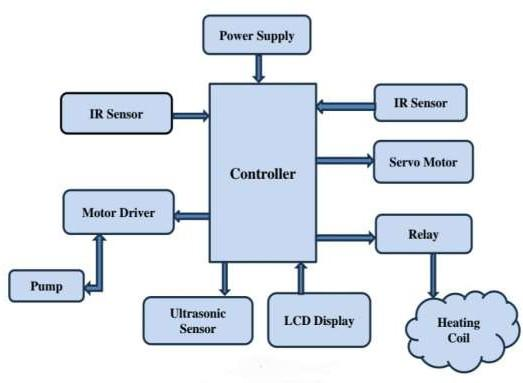
\includegraphics[width=5.4429in,height=3.9898in]{DocumentfromPrachiTorave-img001.jpg}
\end{center}
\clearpage\setcounter{page}{1}\pagestyle{Convertedxix}
{\centering
[Warning: Draw object ignored]\textbf{Chapter VIII:}
\par}

\section[Outcome]{Outcome}

\bigskip


\bigskip

\textcolor{black}{The successful implementation of the IoT-based incinerator project, featuring an optimized heat burner
system, promises a transformative impact on waste management practices. The integration of real-time monitoring and
control, coupled with advanced combustion technologies, leads to a notable improvement in operational efficiency. This
results in enhanced waste reduction, increased energy recovery, and significant cost savings. The system's capacity for
remote monitoring not only adds operational flexibility but also fosters a safer and more responsive waste management
environment. By incorporating emissions control measures, the project ensures compliance with environmental
regulations, contributing to a substantial reduction in harmful pollutants. The project's technological sophistication
positions the waste management facility as a pioneering entity, showcasing a commitment to sustainable practices.
Furthermore, the positive environmental impact, along with adaptability and scalability, makes the project a model for
addressing diverse waste management challenges. Ultimately, the successful execution of this project not only marks a
technological advancement in waste disposal but also underscores a commitment to environmental responsibility and
innovation in the broader context of sustainable development.}


\bigskip


\bigskip


\bigskip

\subsection{Improved Efficiency:}
\textcolor{black}{The real-time monitoring and control capabilities of the IoT system, coupled with an optimized heat
burner, can significantly enhance the efficiency of the incineration process. This leads to better waste reduction,
increased energy recovery, and overall improved operational performance.}

\subsection{Emissions Reduction:}
\textcolor{black}{By implementing advanced combustion technologies and emissions control measures, the project can
contributeto a substantial reduction in harmful emissions. This outcome aligns with environmental regulations and
promotesa more sustainable waste management solution.}

\subsection{Cost Savings:}
\textcolor{black}{The enhanced efficiency and remote monitoring capabilities can result in cost savings. Reduced
operational costs, lower maintenance expenses, and optimized fuel consumption contribute to a more economically viable
waste management system.}

\clearpage\setcounter{page}{1}\pagestyle{Convertedxx}
\section[Chapter]{[Warning: Draw object ignored]Chapter}
{\centering
\textbf{IX:}
\par}


\bigskip

\section[Conclusion]{Conclusion}

\bigskip

\textcolor{black}{In conclusion, the IoT-based incinerator project, featuring an optimized heat burner system,
represents a significant leap forward in waste management practices. The successful implementation of this project
yields a multitude of positive outcomes, including enhanced operational efficiency, emissions reduction, and
substantial cost savings. The integration of real-time monitoring and remote control capabilities not only improves
operational flexibility but also positions the facility at the forefront of technological innovation. By complying with
environmental regulations and incorporating advanced combustion technologies, the project underscores a commitment to
sustainability and responsible waste disposal practices. The positive environmental impact, adaptability, and
scalability of the system make it a model solution for diverse waste management challenges. Overall, the project's
successful execution not only signifies a technological advancement in waste management but also reflects a dedication
to environmental responsibility, innovation, and the pursuit of sustainable development.}

\textcolor{black}{The proposed system serves as a prototype for an automatic slot machine, and after testing the
controller component, it was found to operate in accordance with the specified requirements. This prototype is designed
for the mechanical implementation of a slot machine, leading to the vending of a product upon coin input. The
{\textquotedbl}STREE SWACHHATA{\textquotedbl} concept allows students to request needed items conveniently. Future
advancements in design and control equipment may lead to vending machines with increased accuracy and efficiency.
Originally focused on cleanliness in rural areas, this initiative often involved the self-dispensing ofsanitary
napkins.}

\clearpage\setcounter{page}{1}\pagestyle{Convertedxxi}
\section[Chapter X: Result and Future]{[Warning: Draw object ignored]Chapter X: Result and Future}
\textbf{Scope}


\bigskip


\bigskip

\section[Results:]{Results:}
\textcolor{black}{The result of the IoT-based incinerator project, with its optimized heat burner system, is a
transformative and efficient waste management solution that brings about tangible benefits. The implemented system
demonstrates improved operational efficiency, evidenced by enhanced waste reduction and increased energy recovery.
Through the integration of advanced combustion technologies and emissions control measures, the project achieves a
notable reduction in harmful pollutants, aligning with stringent environmental regulations. The cost savings realized,
coupled with the system's adaptability and scalability, make it a practical and economically viable solution for waste
management challenges. Remote monitoring capabilities add a layer of convenience and responsiveness to operations,
contributing to overall safety and system reliability. Beyond these technical achievements, the successful outcome of
the project positions the waste management facility as a leader in sustainable practices, showcasing a commitment to
environmental responsibility and innovation. In essence, the result is a technologically advanced, environmentally
conscious, and economically sustainable waste management system that stands as a model for addressing contemporary
waste disposal challenges.}


\bigskip


\bigskip

\subsection{Working Model:}

\bigskip


\bigskip


\bigskip


\bigskip


\bigskip


\bigskip


\bigskip


\bigskip


\bigskip


\bigskip


\bigskip


\bigskip


\bigskip

\textbf{Fig 8: IOT Based Incinerator Working Model}

\clearpage\setcounter{page}{1}\pagestyle{Convertedxxii}
\section[Future Scope:]{[Warning: Draw object ignored]Future Scope:}

\bigskip


\bigskip

\subsection{Integration of Artificial Intelligence (AI):}
\textcolor{black}{Incorporating AI algorithms can enhance the system's predictive capabilities, allowing it to learn and
adapt to changing waste compositions and operational conditions over time.}

\subsection{Energy Recovery Optimization:}
\textcolor{black}{Future iterations of the project could focus on further optimizing energy recovery processes,
exploring innovative ways to harness and utilize the heat generated during incineration for additional energy needs.}

\subsection{Waste Sorting and Segregation Integration:}
\textcolor{black}{Integrating IoTtechnologies to monitor and control waste sorting and segregation processes can
contribute to more precise incineration, ensuring that materials are incinerated at optimal conditions.}

\subsection{Advanced SensorTechnologies:}
\textcolor{black}{The incorporation of state-of-the-art sensor technologies, such as hyperspectral sensors, could
provide even more detailed information about waste composition, enabling finer controlover combustion processes.}

\subsection{Blockchain forAccountability:}
\textcolor{black}{Implementing blockchain technology could enhance transparency and accountability in waste management,
providing an immutable record of waste disposal and emission reduction efforts.}

\clearpage\setcounter{page}{1}\pagestyle{Convertedxxiii}
\section[Chapter XI: References]{[Warning: Draw object ignored]Chapter XI: References}

\bigskip


\bigskip

\liststyleWWNumix
\begin{enumerate}
\item \textcolor{black}{Fan Bai, Xiaochang Wang, (2011) Nitrogen Holding Propertyof the Composts in an Aerobic
Mesophilic Composting Reactor for Sanitary Disposal of Human Feces, IEEE, vol.7, issue 11,.}
\item \textcolor{black}{Jogdand K, Yerpude PA, (2011). Community based study on menstrual hygiene among adolescent
girls.}
\end{enumerate}

\bigskip

\textcolor{black}{Indian Journal of Matern Child Health, Vol. 13, 1-6.}

\liststyleWWNumix
\setcounter{saveenum}{\value{enumi}}
\begin{enumerate}
\setcounter{enumi}{\value{saveenum}}
\item \textcolor{black}{Suhail, Beg, (2014) ``Implementation of FSM Based Automatic Dispense Machine with Expiry Date
Feature Using VHDL,'' International Journal of Modern Engineering Research (IJMER), vol. 4, p.p. 1- 5.}
\item \textcolor{black}{Singh, (2015) ``Touch Screen Based Automated Medical Vending Machine,'' International Journal
for Innovative Research in Science \& Technology (IJIRST), vol. 1, p.p. 1-4.}
\item \textcolor{black}{Linda scott, paul Montgomery, laurel stinfielt, Catherine dolan, (2013) Sanitary Pad
Acceptabilityand Sustainability Study, University of Oxford.}
\end{enumerate}

\bigskip


\bigskip

\liststyleWWNumix
\setcounter{saveenum}{\value{enumi}}
\begin{enumerate}
\setcounter{enumi}{\value{saveenum}}
\item \textcolor{black}{Das, N., Mandal, R., Mitra, A., Maiti, B., Nandy, S., and Datta, D. (2018). FPGABased Vending
Machine.}
\item \textcolor{black}{Hossain, S., and Sen, V. (2018). Factors Influencing Hygienic Practices During Menses Among
Girls}
\end{enumerate}
\textcolor{black}{From Jaipur, Rajasthan. International Journal Of Scientific Research, 6(11).}

\liststyleWWNumix
\setcounter{saveenum}{\value{enumi}}
\begin{enumerate}
\setcounter{enumi}{\value{saveenum}}
\item \textcolor{black}{Rotary Club of kalyan, Sanitary Napkin Vending Machines and Disposal Machines for Girls in
RuralArea School and College.}
\end{enumerate}
\clearpage\setcounter{page}{1}\pagestyle{Convertedxxiv}
\section[Chapter XI: Expenditure]{[Warning: Draw object ignored]Chapter XI: Expenditure}

\bigskip


\bigskip


\bigskip

\begin{flushleft}
\tablefirsthead{}
\tablehead{}
\tabletail{}
\tablelasttail{}
\begin{supertabular}{|m{0.9851598in}|m{3.3351598in}|m{1.7615598in}|}
\hline
\textbf{\textcolor{black}{Sr.No.}} &
\textbf{\textcolor{black}{Items}} &
\textbf{\textcolor{black}{Cost (Rs)}}\\\hline
\textcolor{black}{1} &
\textcolor{black}{Node MCU ESP 8266} &
\textcolor{black}{450}\\\hline
\textcolor{black}{2} &
\textcolor{black}{Ultrasonic Sensor} &
\textcolor{black}{140}\\\hline
\textcolor{black}{3} &
\textcolor{black}{LCD Display 16*2} &
\textcolor{black}{160}\\\hline
\textcolor{black}{4} &
\textcolor{black}{I2C Model} &
\textcolor{black}{110}\\\hline
\textcolor{black}{5} &
\textcolor{black}{IR Sensor} &
\textcolor{black}{55}\\\hline
\textcolor{black}{6} &
\textcolor{black}{Relay Model} &
\textcolor{black}{55}\\\hline
\textcolor{black}{7} &
\textcolor{black}{Servo Motor} &
\textcolor{black}{250}\\\hline
\textcolor{black}{8} &
\textcolor{black}{Arduino UNO} &
\textcolor{black}{650}\\\hline
\textcolor{black}{9} &
\textcolor{black}{Switch} &
\textcolor{black}{50}\\\hline
\textcolor{black}{10} &
\textcolor{black}{Battery} &
\textcolor{black}{800}\\\hline
\textcolor{black}{11} &
\textcolor{black}{PUMP} &
\textcolor{black}{95}\\\hline
\textcolor{black}{12} &
\textcolor{black}{Heating Burner} &
\textcolor{black}{7500}\\\hline
~
 &
~

\centering \textbf{\textcolor{black}{Total}} &
~

\centering\arraybslash \textbf{\textcolor{black}{10,335}}\\\hline
\end{supertabular}
\end{flushleft}

\bigskip
\end{document}
